\begin{figure}[H]
    \centering
    \begin{subfigure}{0.48\textwidth}
        \centering
        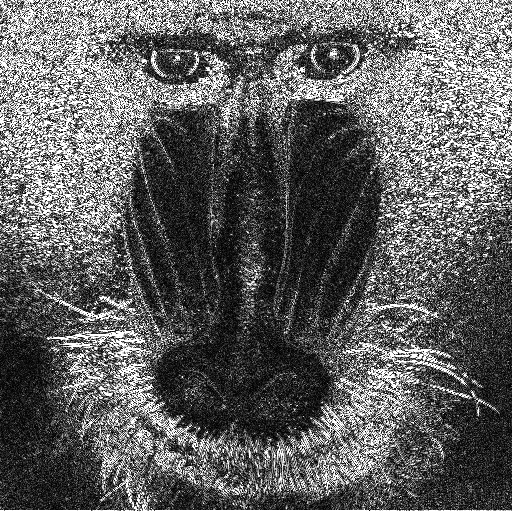
\includegraphics[width=0.9\textwidth]{imagens/baboon.png}
        \caption{Original: \texttt{baboon.png}.}
    \end{subfigure}\\[8pt]
    \begin{subfigure}{0.48\textwidth}
        \centering
        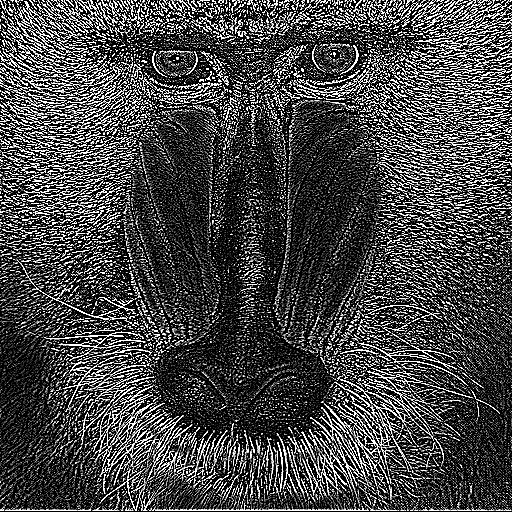
\includegraphics[width=0.9\textwidth]{resultados/baboon_h1.png}
        \caption{Convolução com $h_1$ (\ref{fig:h1}).}
        \label{fig:borda:viz4}
    \end{subfigure}%
    \begin{subfigure}{0.48\textwidth}
        \centering
        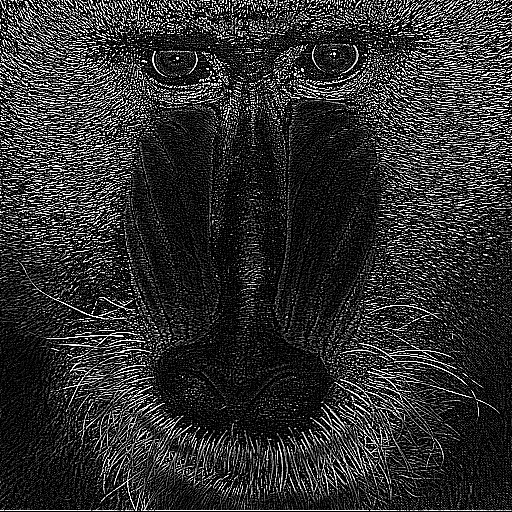
\includegraphics[width=0.9\textwidth]{resultados/baboon_h5.png}
        \caption{Convolução com $h_5$ (\ref{fig:h5}).}
        \label{fig:borda:viz8}
    \end{subfigure}

    \caption{Aplicação do laplaciano discreto.}
\end{figure}

Os filtros de detecção ou realce de bordas mais comuns são os chamados não-direcionais. Normalmente, eles são desenvolvidos a partir do operador laplaciano discreto \autocite{ref:laplacian}. Uma característica importante dos filtros de detecção de bordas é que seus elementos somam zero.

O operador laplaciano serve como uma medida de quanto uma função espacial no ponto $p$ é diferente da média dos pontos em um raio $[p - \delta r, p + \delta r]$. No caso discreto bidimensional, como imagens, existem duas principais medidas de distância, considerando a vizinhaças 4 e 8. Elas resultam em dois tipos de laplacianos diferentes, como pode ser visto na \cref{fig:borda:kernel}.

Nesse trabalho temos o \textit{kernel} $h_1$ (\ref{fig:h1}), com vizinhaça 4 de raio 2, e o $h_5$, com vizinhaça 8 de raio 1. Os resultados podem ser vistos nas figuras \ref{fig:borda:viz4} e \ref{fig:borda:viz8}, respectivamente. Podemos ver que as bordas nas regiões de baixa frequência são bem detectadas, como no centro da imagem, mas regiões de alta frequência resultam em muita informação e podem acabar atrapalhando a análise das bordas. Uma forma de contorna esse problema é aplicando um filtro passa-baixas, como o \textit{blur} gaussiano, discutido na \cref{sec:blur}.

\begin{figure}[H]
    \centering
    \begin{subfigure}{0.4\textwidth}
        \centering
        \begin{kmatrix}
    \matrix[square matrix]{
        0 & 0 & -1 & 0 & 0 \\
        0 & -1 & -2 & -1 & 0 \\
        -1 & -2 & 16 & -2 & -1 \\
        0 & -1 & -2 & -1 & 0 \\
        0 & 0 & -1 & 0 & 0 \\
    };
\end{kmatrix}
        \caption{~$h_1$}
        \label{fig:h1}
    \end{subfigure}%
    \begin{subfigure}{0.4\textwidth}
        \centering
        \begin{kmatrix}
    \matrix[square matrix]{
        -1 & -1 & -1 \\
        -1 & 8 & -1 \\
        -1 & -1 & -1 \\
    };
\end{kmatrix}
        \caption{~$h_5$}
        \label{fig:h5}
    \end{subfigure}

    \caption{Filtros laplacianos discretos}
    \label{fig:borda:kernel}
\end{figure}

A execução pode ser feita com:

\begin{minted}{bash}
    $ python3 main.py imagens/baboon.png h1
    # ou
    $ python3 main.py imagens/baboon.png h5
\end{minted}
